\subsection{Software Environment}

\centeredlargetext{white}{black}{
Software Environment
}

{
\setbeamertemplate{background}{}
\begin{frame}
\frametitle{Welcome to Ubuntu GNU/Linux}
\begin{center}

\includegraphics[height=0.5\paperheight]{../Art/Tux.png}

\includegraphics[width=0.5\paperwidth]{../Art/blackeubuntulogo.png}
\end{center}
\end{frame}
}

{
\setbeamertemplate{background}{}
\begin{frame}
\frametitle{How to take the mouse out of the Virtual Machine}
\begin{itemize}
\item Hit the \textbf{RIGHT CTRL} Key on Windows / Linux Host
\item Hit the \textbf{LEFT APPLE} Key on Mac Host
\end{itemize}
\end{frame}
}

{
\setbeamertemplate{background}{}
\begin{frame}
\frametitle{How to Open a Terminal - Icon in Upper Left Corner}
\framesubtitle{To type your command line instructions}
\begin{center}
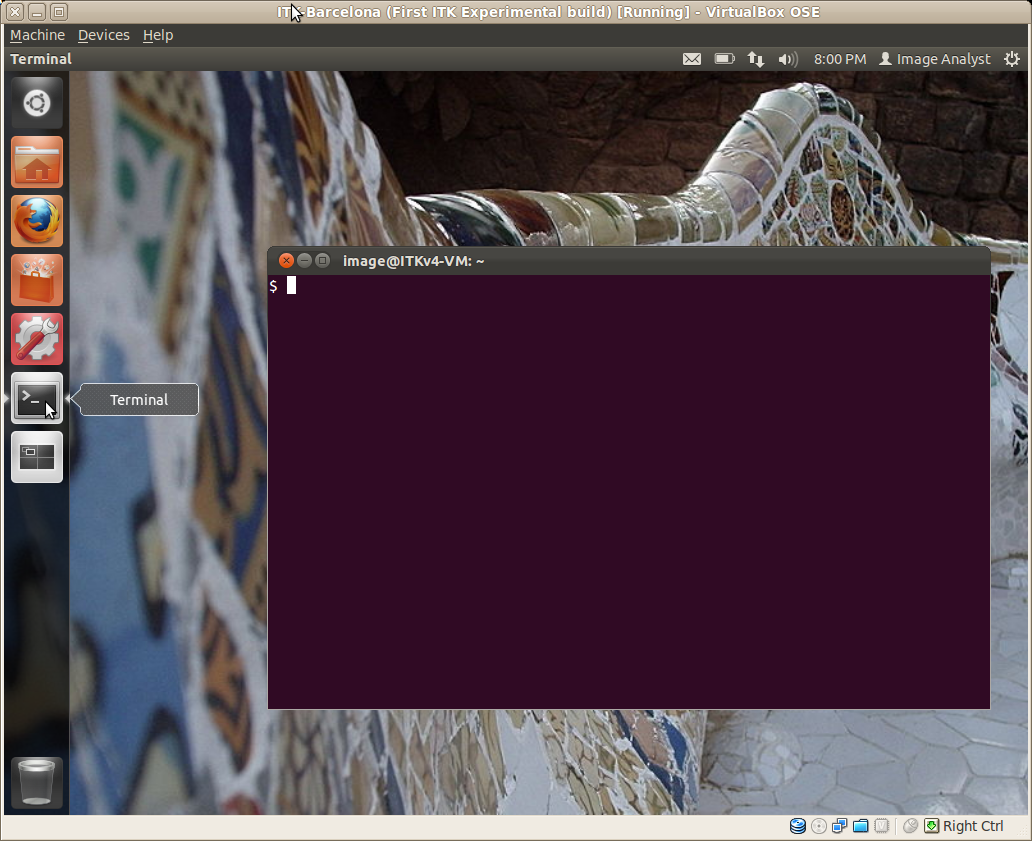
\includegraphics[width=0.7\paperwidth]{../Art/Screenshot-OpenTerminal.jpg}
\end{center}
\end{frame}
}

{
\setbeamertemplate{background}{}
\begin{frame}
\frametitle{How to Navigate Directories}
\framesubtitle{Double Click in Folder Icons in the Desktop}
\begin{center}
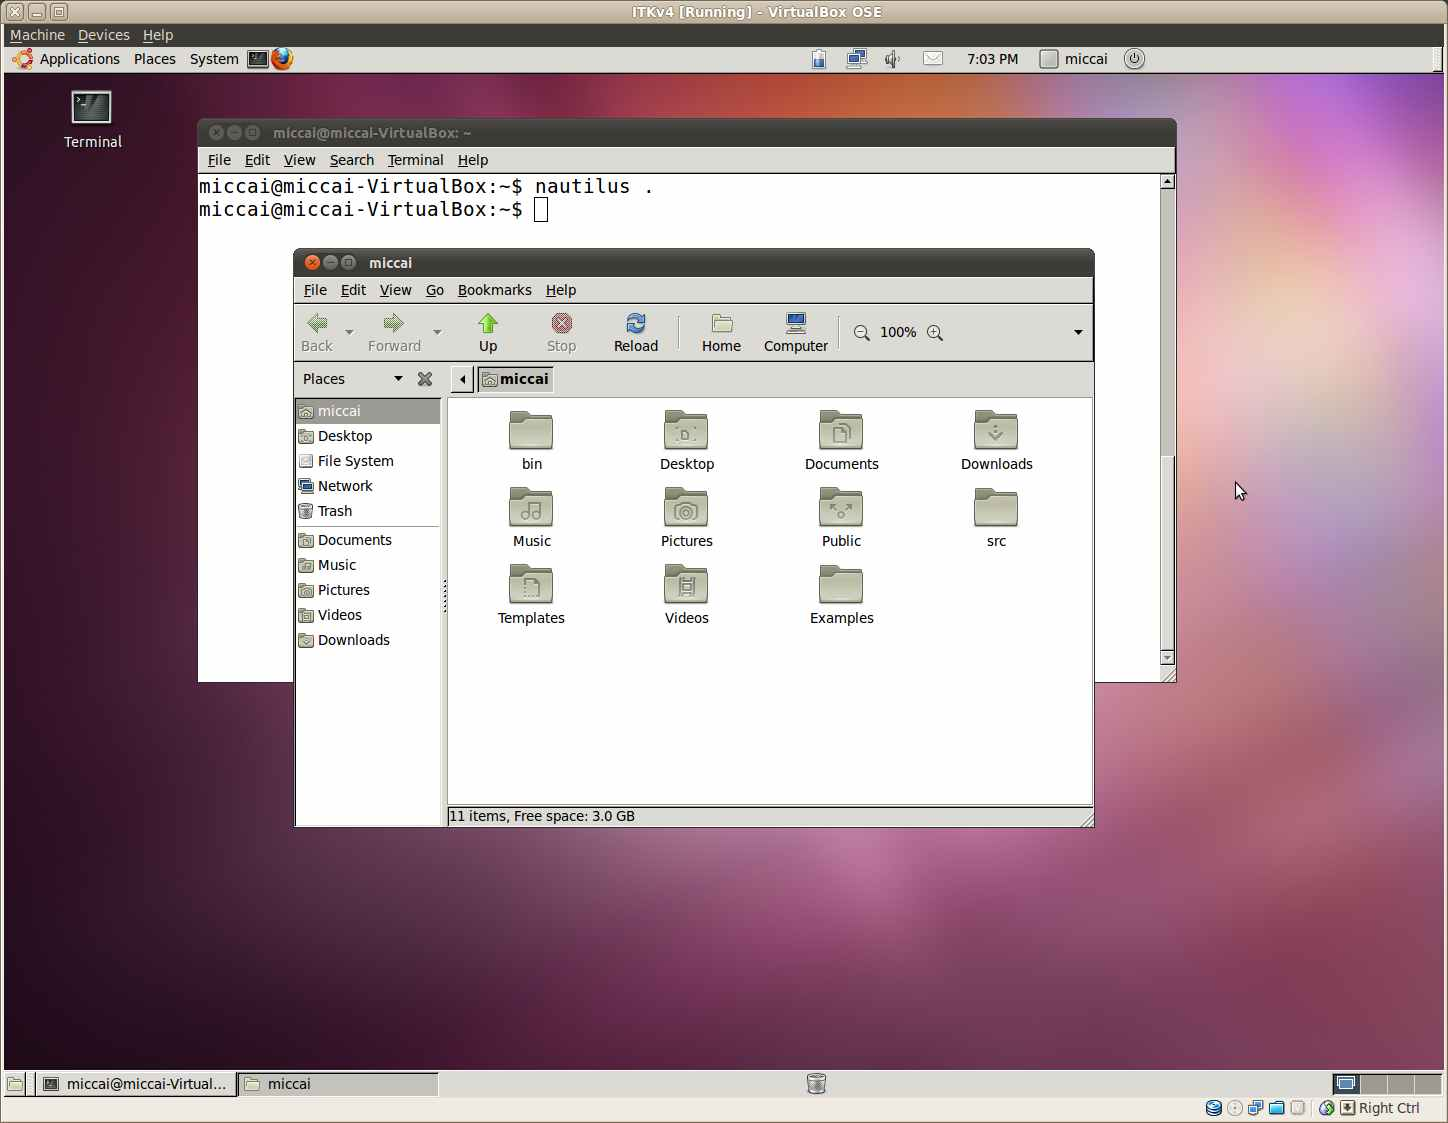
\includegraphics[width=0.7\paperwidth]{../Art/Screenshot-Nautilus.jpg}
\end{center}
\end{frame}
}

{
\setbeamertemplate{background}{}
\begin{frame}[fragile]
\frametitle{Walk through the directories}
\begin{itemize}
\item Find source code of exercises
\begin{verbatim}
cd ~/src/ITKv4-TheNextGeneration-Tutorial/Exercises
pwd
ls
nautilus .
\end{verbatim}
\pause
\item Find binary build of exercises
\begin{verbatim}
cd ~/bin/ITKv4-TheNextGeneration-Tutorial/Exercises
pwd
ls
\end{verbatim}
\end{itemize}
\end{frame}
}

{
\setbeamertemplate{background}{}
\begin{frame}[fragile]
\frametitle{How to View Images}
\begin{itemize}
\item Go to the directory
\item Invoke ``eye of gnome" eog application
\begin{verbatim}
cd ~/src/ITK/Examples/Data/
eog BrainProtonDensitySlice.png
\end{verbatim}
\pause
\item Hit ESC key to quit the application
\end{itemize}
\end{frame}
}
